
\subsection{Ecualización de histogramas}

Una variable aleatoria cuya distribución es uniforme tiene la misma probabilidad
de realizarse con un valor, que con cualquier otro. Sin embargo, si se
uniformiza el histograma para que todos los valores de luminancia sean
equiprobables, se perdería la característica de la imagen y el resultado
carecería de sentido en comparación a la original. Es por ello que se
recurre a la linealización de la función de densidad acumulada $F_X(X)$.

De esta manera, al uniformizar la densidad, los picos de luminancia se esparcen
para no quedar concentrados en un rango acotado, aumentando el contraste. \\

Dada una imagen digital de $N$ píxeles con un rango de $M$ valores de luminancia
(típicamente $M=256$) se puede estimar la función densidad de probabilidad de
la luminancia $x$ (\emph{PDF}, \emph{probability density function}) según:

\begin{equation} \label{eq:pdf}
	f(x) = \sum_{i=0}^{M-1} \frac{n_i}{N} \; \mathds{1} \left\{ x = x_i \right\}
\end{equation}

donde $n_i$ corresponde a la cantidad de píxeles cuya luminancia es $x_i$ (que
se limita a $M$ niveles). Éste es el fundamento detrás del uso de histogramas
que representan la \emph{PDF} en un gráfico de barras generado a partir de la
ecuación \eqref{eq:pdf}.

Luego, se obtiene la función de densidad acumulada (\emph{CDF, cumulative
density function}):

\begin{equation} \label{eq:cdf}
	F_X(X) = \sum_{i=0}^{M-1} f(x) \; \mathds{1} \left\{ x \leq x_i \right\}
\end{equation}

Ahora, a partir de la \emph{CDF} calculada en la ecuación \eqref{eq:cdf}, se
realiza el ajuste de la imagen a través de \emph{HE} operando según la siguiente
ecuación para cada píxel ${pix}_i$:

\begin{equation} \label{eq:he_full}
	\textit{HE } ({pix}_i) = \frac{R \; \left[f({pix}_i) - \min\{f(x)\}\right]}{\max\{f(x)\}-\min\{f(x)\}}
\end{equation}

En nuestro caso particular, donde se busca un rango máximo, $R = M - 1 = 255$,
$\max\{f(x)\} = 1$ y $\min\{f(x)\} = 0$. Por lo tanto la ecuación
\eqref{eq:he_full} se puede simplificar:

\begin{equation} \label{eq:he}
	\textit{HE } ({pix}_i) = 255 \cdot f({pix}_i)
\end{equation}

Así, cada valor de luminancia se mapea según su \emph{CDF} a un nuevo valor de
luminancia, manteniendo la posición espacial original.

\graficarMulticolPNG{graph_comp_hist_og_he}{Ejemplo comparativo de histogramas de imágenes con y sin ecualización.}{fig:comp_hist_og_he}

Como se puede ver en la siguiente comparación entre la imagen original y la
ajustada, ésta última realza en exceso el contraste de la imagen generando
efectos indeseados como por ejemplo nubes borrosas de píxeles sobre el personaje
o en los arbustos.

\noindent
\begin{minipage}{\columnwidth}
	\makeatletter
	\newcommand{\@captype}{figure}
	\makeatother
	\centering
		\subfloat[\emph{Original}]{%
			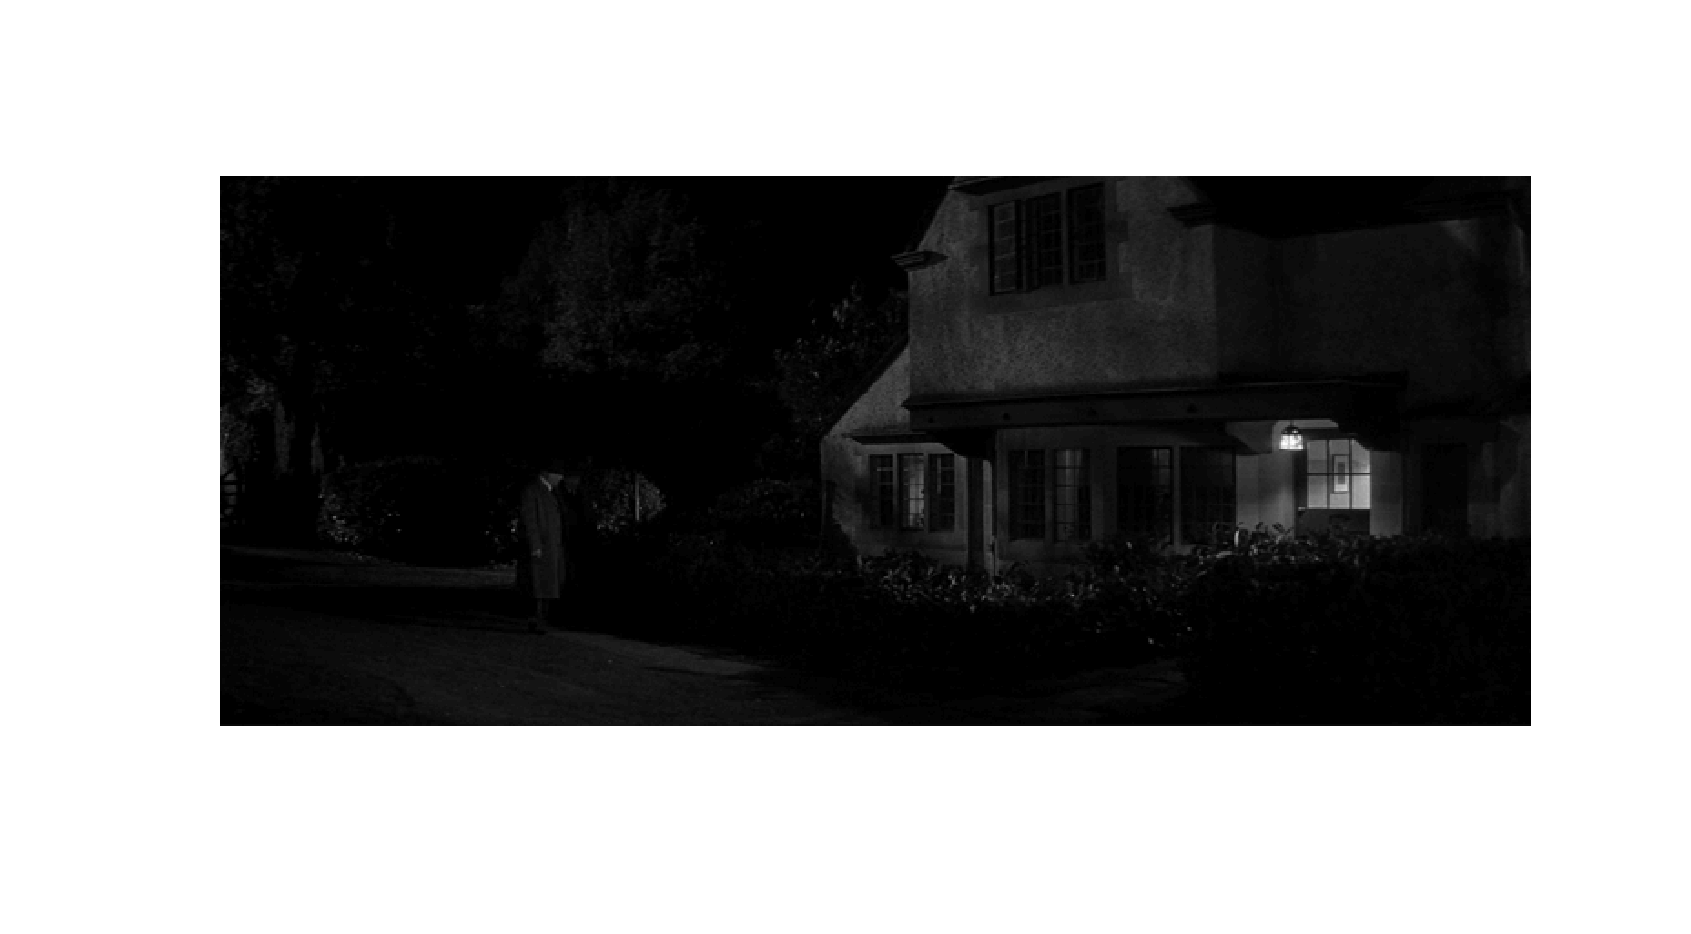
\includegraphics[width=1.0\textwidth]{result_orig_shadowlands}%
			\label{fig:im_orig_he}%
		}\qquad%
		\subfloat[\emph{HE}]{%
			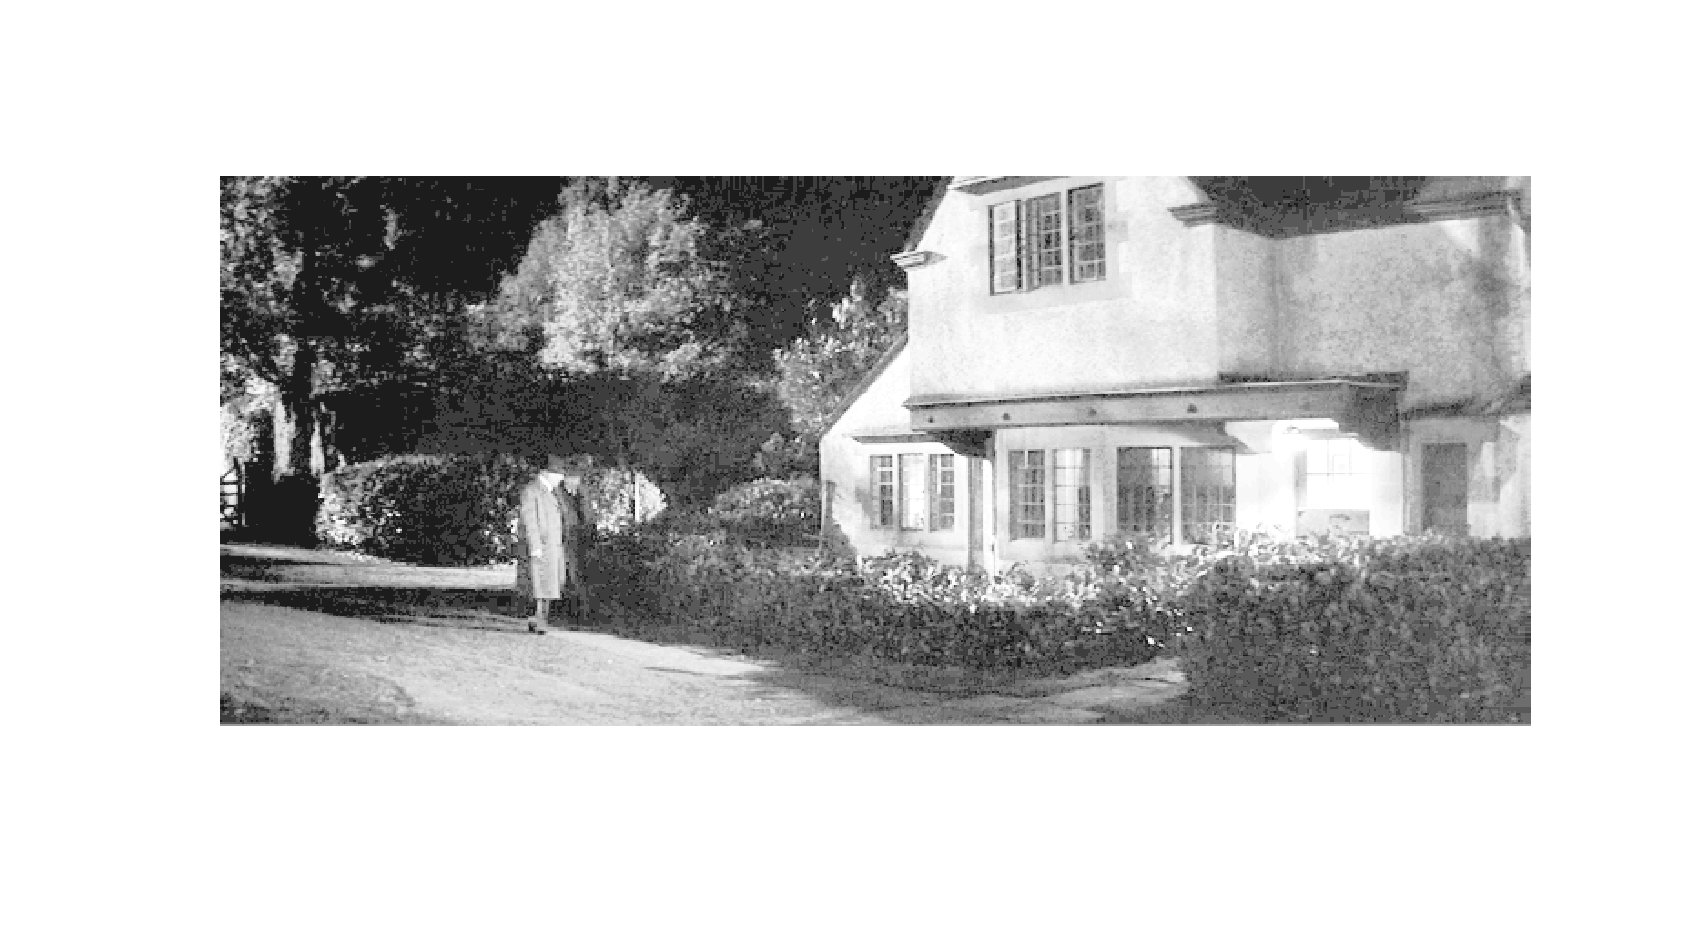
\includegraphics[width=1.0\textwidth]{result_he_shadowlands}%
			\label{fig:im_eq_he}%
		}
	\caption{\emph{Imágenes con y sin HE.}}
\end{minipage}
